%!TEX program = pdflatex
% Full chain: pdflatex -> bibtex -> pdflatex -> pdflatex
\documentclass[11pt,en]{elegantpaper}

\title{Investigación reproducible \\ Buenas prácticas para el manejo de datos y códigos\footnote{Traducción al español a cargo de: Sebastián Hernández y Rony Rodríguez-Ramírez.}}
\author{Harrison Diamond Pollock \and Erica Chuang \and Stephanie Wykstra}
\date{\today}


\begin{document}
%----------------------------------------------------------------------------------------
\maketitle
\tableofcontents
%----------------------------------------------------------------------------------------
\newpage 
%----------------------------------------------------------------------------------------
\section{Introducción}
\label{sec:intro}

Las revistas, los financiadores de investigación y los grupos de investigación como Innovations for Poverty Action reconocen cada vez más el valor de la transparencia en la investigación. La transparencia de la investigación incluye el registro previo de estudios y el intercambio de materiales como datos y códigos para permitir que otros vuelvan a analizar los resultados informados.

La gestión adecuada de datos y códigos durante un proyecto es esencial para la transparencia después de la finalización de un proyecto. También son importantes para uso interno, ya que los proyectos a menudo se ejecutan durante varios años, con varios miembros del personal trabajando en ellos de forma secuencial.

Esta guía describe las mejores prácticas en el manejor de datos y códigos. El alcance de la guía es cubrir los principios de organización y documentación de materiales en todos los pasos del ciclo de vida de un proyecto con el objetivo de hacer que la investigación sea reproducible. La guía no cubre las mejores prácticas para diseñar encuestas, limpiar datos o realizar análisis de datos. En cada sección, explicamos el "qué", el "por qué" y el "cómo" de cada práctica recomendada.

Para comentarios/preguntas, comuníquese con \href{mailto:researchsupport@poverty-action.org}{researchsupport@poverty-action.org}.
%----------------------------------------------------------------------------------------
\newpage 
\section{Estructura de carpetas y archivos}
\label{sec:estructura}
%----------------------------------------------------------------------------------------
\textbf{¿Qué?}

La estructura de carpetas describe la organización de las carpetas que contienen todos los archivos del proyecto. Por lo general, las carpetas se designan para ciertos tipos de archivos (e.g., do-files, archivos de datos, tablas, etc.), así como puntos en el tiempo (e.g., línea de base, línea media, línea final).

\textbf{¿Por qué?} 

Mantener una estructura de carpetas lógica significa que es mucho más fácil encontrar los archivos que está buscando. También facilita enormemente compartir un proyecto con otras personas, como los investigadores principales (PI, por sus siglas en inglés) y los nuevos asistentes de investgiación (RA, por sus siglas en inglés) que trabajan en un proyecto. Tener un conjunto desorganizado de archivos significa que las transiciones de proyectos se vuelven mucho más difíciles


\textbf{¿Cómo?}

\hyperref[fig:carpetas]{Aquí} un ejemplo de una estructura de carpetas describe una división lógica de archivos para un proyecto de investigación completo, y \hyperref[fig:code]{aquí} hay una estructura de carpetas recomendada para archivos de datos y códigos. 

Independientemente de la estructura de carpetas específica que usted decida, es fundamental \textbf{definirla de antemano} y limitar los archivos que necesita mantener (especialmente las base de datos) solo a aquellos que son estrictamente necesarios. Si desea mantener archivos extras/antiguos, es una buena práctica crear una carpeta "Archivo" donde se almacenan. \hyperref[sec:doorganizar]{Ver más abajo}.

¿Qué hay de heredar una estructura de carpetas existente? Si bien el caso ideal sería reorganizar los archivos y carpetas para que se ajusten a una estructura como la descrita anteriormente, es probable que sea un paso poco práctico y que requiera mucho tiempo. Antes de realizar cualquier cambio, un RA necesitaría un amplio conocimiento de la estructura actual y la relación entre los archivos. Crear un \textbf{mapa de carpetas} es una práctica recomendable en este caso. Este mapa (en Excel/Word) resumiría las carpetas clave en la estructura y qué archivos se encuentran dentro de ellas. Dicho documento formaría la base del \href{http://www.poverty-action.org/research-transparency/example-readme-files}{ReadME} del proyecto y resultará útil durante todo el ciclo de vida del proyecto.

\textbf{Nota:} Mantenga los nombres de archivos y carpetas simples y, siempre que sea posible, sin espacios.
%----------------------------------------------------------------------------------------
\section{Mejores prácticas para códigos}
\label{sec:practicas}
%----------------------------------------------------------------------------------------

%----------------------------------------------------------------------------------------
\subsection{Nombrar y etiquetar variables}
\label{sec:variables}
%----------------------------------------------------------------------------------------
\textbf{¿Qué?}


\textbf{¿Por qué?} 


\textbf{¿Cómo?} 
%----------------------------------------------------------------------------------------
\subsection{Manejo de valores perdidos}
\label{sec:missings}
%----------------------------------------------------------------------------------------
\textbf{¿Qué?}


\textbf{¿Por qué?}


\textbf{¿Cómo?}
%----------------------------------------------------------------------------------------
\subsection{Escribiendo do-files}
\label{sec:dofiles}
%----------------------------------------------------------------------------------------

%----------------------------------------------------------------------------------------
\subsection{Cómo escribir un do-file maestro}
\label{sec:domaestro}
%----------------------------------------------------------------------------------------

%----------------------------------------------------------------------------------------
\subsection{Cómo organizar y referenciar do-files}
\label{sec:doorganizar}
%----------------------------------------------------------------------------------------

%----------------------------------------------------------------------------------------
\subsection{Usando referencias relativas}
\label{sec:refrelativas}
%----------------------------------------------------------------------------------------

%----------------------------------------------------------------------------------------
\newpage 
\section{Mantener un buen código y documentación de datos}
\label{sec:documentacion}
%----------------------------------------------------------------------------------------
\textbf{¿Qué?}

Mantener su código y sus datos bien documentados significa mantener organizados todos los archivos asociados con su proyecto y rastrear todas las decisiones clave con respecto a ellos. También significa describir la relación entre sus datos y código (e.g., en un archivo ReadME) y cualquier otro archivo importante.

\textbf{¿Por qué?}

Una buena documentación es esencial cada vez que alguien además del autor original quiere comprender o ampliar el trabajo existente. Incluso para el autor, a menudo es difícil hacer un seguimiento de los archivos que pueden haberse creado o de las decisiones que se tomaron incluso unas pocas semanas antes. Mantener un buen registro de estos problemas será de gran ayuda para aliviar problemas futuros y hará que un proyecto sea mucho más propenso a ser utilizado por otros de manera efectiva.

\textbf{¿Cómo?}

Un aspecto clave de una buena documentación es un archivo ReadMe. Este archivo (a menudo en PDF o Word) puede adoptar una variedad de formas y longitudes, pero como mínimo, debe describir el código clave y los archivos de datos del proyecto y cómo interactúan. Puede encontrar algunos archivos ReadMe me muestra \href{http://www.poverty-action.org/research-transparency/example-readme-files}{aquí}. Además, los archivos ReadMe pueden incluir información sobre cualquier comando escrito por un usuario (también es una buena práctica incluirlos en un \href{http://www.poverty-action.org/research-transparency/example-master}{do-file maestro} como parte del encabezado), así como pautas sobre la interpretación de variables o procesos particulares. Tenga en cuenta que la información de implementación/logística del proyecto también debe rastrearse, pero se debe mantener en un documento separado la información sobre datos y código.

Si bien generalmente uno publicaría un archivo ReadMe junto con los datos y código, \textbf{es fundamental hacer que el archivo ReadMe sea un documento vivo.} Es decir, que se actualice a lo largo del ciclo de vida del proyecto. Este "registro vivo" debe actualizarse regularmente con notas importantes sobre archivos y variables según sea necesario. Como se enfatizó, esto hace que trabajar en un proyecto existente sea mucho más fácil, además de ser un recurso clave cuando se comparte.

La buena documentación también se hace mucho más fácil con una organización de archivos efectiva. Consulte la sección anterior - Estructura de carpetas y archivos - para obtener más información. Particularmente para el trabajo colaborativo en código, considere usar \href{https://github.com/}{GitHub}. GitHub es una plataforma web que facilita la escritura colaborativa de códigos, así como el seguimiento de versiones y tareas. La plataforma puede facilitar en gran medida el seguimiento de archivos e información sobre ellos a lo largo del tiempo. IPA ha compilado algunas herramientas para aprender y usar GitHub, que se pueden encontrar \href{https://github.com/PovertyAction/github-training}{aquí}. (¡Tenga en cuenta que nuestros recursos de GitHub están en GitHub!) Vaya a la \href{https://github.com/PovertyAction/github-training/blob/master/resources/GitHub\%20User\%20Guide.md}{Guía del usuario de GitHub} para obtener instrucciones sobre cómo comenzar a utilizar la plataforma.

Algunas características importantes a tener en cuenta:

\begin{itemize}
	\item Los grupos de archivos se pueden "etiquetar" en cualquier momento de la historia, de modo que uno pueda volver fácilmente, digamos, a los archivos tal como estaban cuando se enviaron por primera vez a una revista para su publicación.
	
	\item Se pueden adjuntar notas y se pueden entablar conversaciones entre múltiples usuarios en archivos individuales y/o líneas de archivos, lo que facilita la exploración de datos importantes sobre un proyecto.
	
	\item Los archivos se pueden comparar fácilmente entre sí para poder visualizar los cambios realizados con el tiempo. Cuando se cargan archivos ("confirmados"), se pueden adjuntar descripciones de los cambios para que exista un registro del proceso de pensamiento en el momento de realizar el cambio.
	
	\item GitHub se puede usar para tareas definidas de forma limitada (e.g., verificaciones de código) o se puede usar de manera más integral para rastrear todos los archivos de proyecto.
\end{itemize}

Si está considerando usar GitHub, comuníquese a \href{mailto:researchsupport@poverty-action.org}{researchsupport@poverty-action.org} con el Soporte de investigación de IPA, y le invitaremos a unirse a la cuenta de \href{https://github.com/PovertyAction}{PovertyAction}, nuestra cuenta organizacional en GitHub (solo para el personal de IPA y sus afiliados).

%----------------------------------------------------------------------------------------
\section{PII y mantener seguros los datos y el código}
\label{sec:pii}
%----------------------------------------------------------------------------------------
\textbf{¿Qué?}


\textbf{¿Por qué?}


\textbf{¿Cómo?} 

%----------------------------------------------------------------------------------------
\newpage 
%----------------------------------------------------------------------------------------
\appendix 
\section{Estructura de las carpetas}
\label{sec:appendix}
%----------------------------------------------------------------------------------------
\begin{figure}[htbp]
	\centering
	\caption{Estructura general de las carpetas del proyecto.\label{fig:carpetas}}
	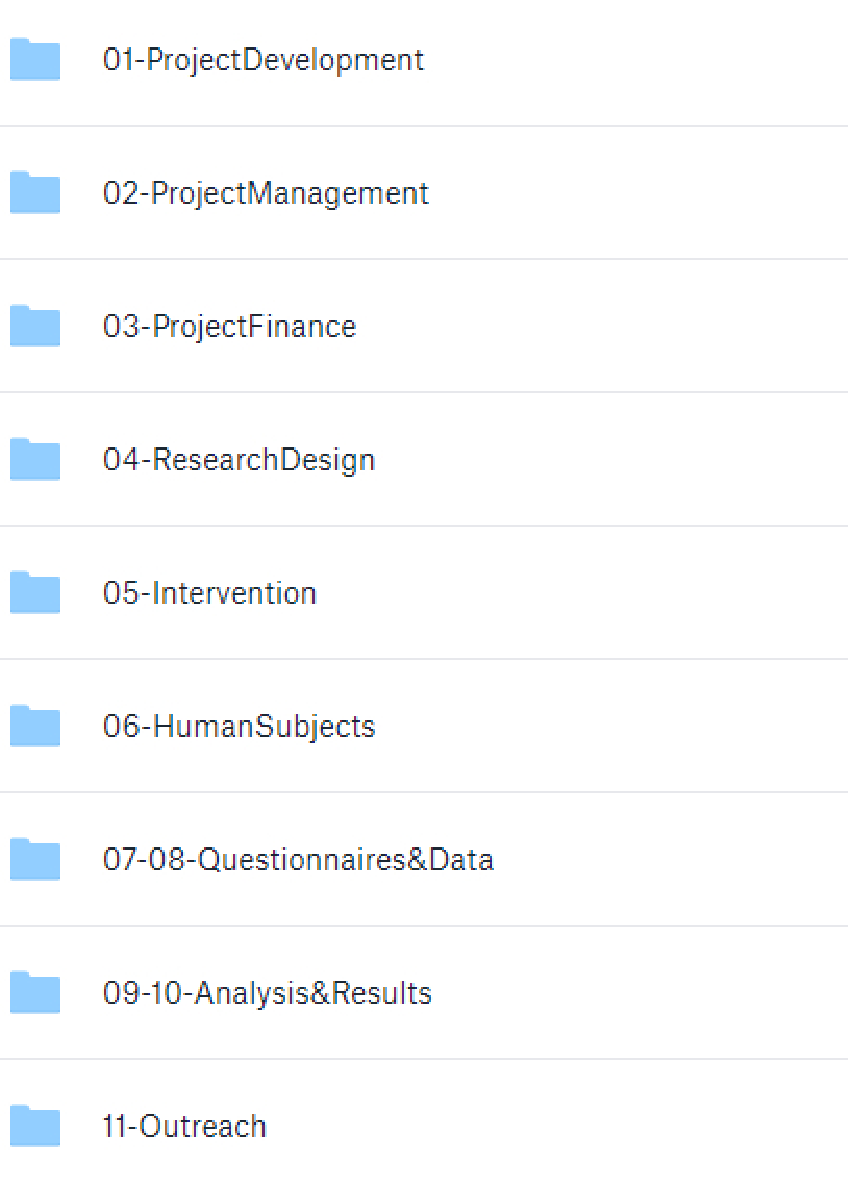
\includegraphics[width=0.35\textwidth]{fig1.pdf}
\end{figure}


\begin{figure}[htbp]
	\centering
	\caption{Estructura de las carpetas de datos y códigos. \label{fig:code}}
	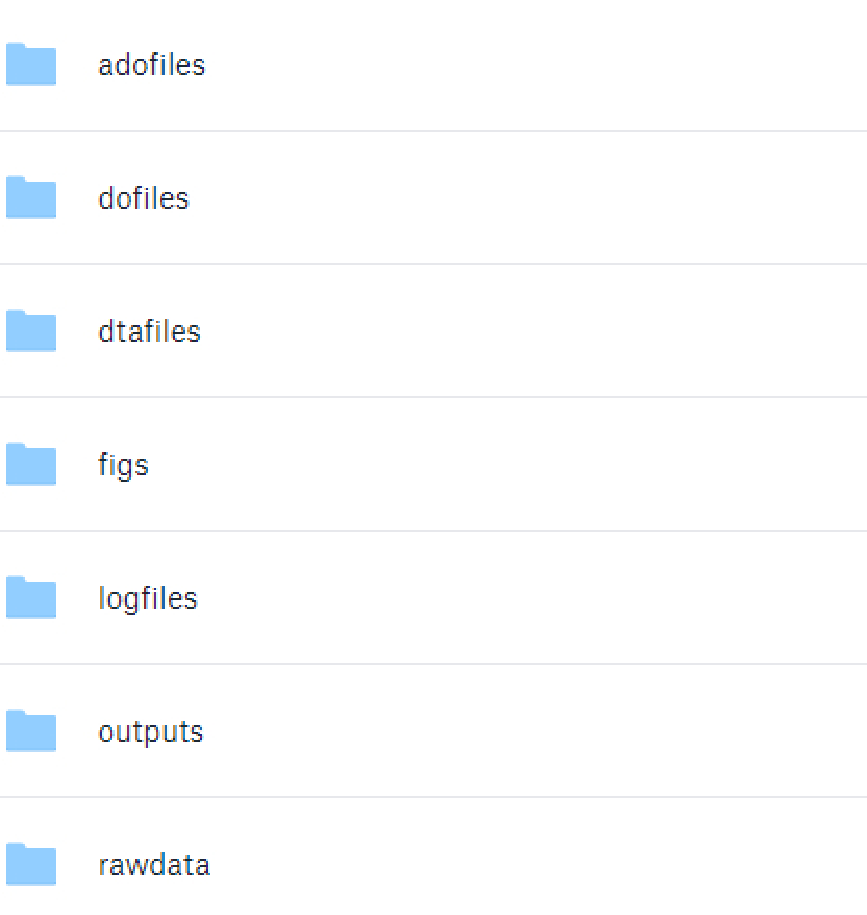
\includegraphics[width=0.35\textwidth]{fig2.pdf}
\end{figure}
\end{document}
%----------------------------------------------------------------------------------------
